\documentclass[border=0.05cm]{standalone}
\usepackage{../../../../preamble_formulas}

\def\eps{0.06}
\def\x{0.05}
\def\sepx{2}

\begin{document}
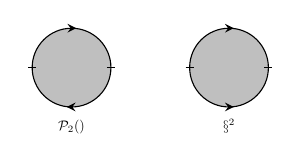
\begin{tikzpicture}
  % Circle 1
  \filldraw[fill=lightgray] (0,0) circle (0.5);

  % Horizontal lines
  \draw (-0.5 -\x,0) -- (-0.5 +\x,0);
  \draw (0.5 -\x,0) -- (0.5 +\x,0);

  % arrows
  \draw [-stealth] (0,0.5) -- (\eps,0.5);
  \draw [-stealth] (0,-0.5) -- (-\eps,-0.5);

  % label
  \node[anchor=north,scale=0.5] at (0,-0.1-0.5) {$\mathcal{P}_2(\RR)$};



  % Circle 2
  \filldraw[fill=lightgray] (\sepx,0) circle (0.5);

  % Horizontal lines
  \draw (\sepx-0.5 -\x,0) -- (\sepx-0.5 +\x,0);
  \draw (\sepx+0.5 -\x,0) -- (\sepx+0.5 +\x,0);

  % arrows
  \draw [-stealth] (\sepx+0,0.5) -- (\sepx+\eps,0.5);
  \draw [-stealth] (\sepx+0,-0.5) -- (\sepx+\eps,-0.5);

  % label
  \node[anchor=north,scale=0.5] at (\sepx,-0.1-0.5) {$\S^2$};
\end{tikzpicture}
\end{document}